\documentclass[a4paper]{article}

\usepackage{graphicx}
\usepackage{amsmath,amssymb}
\usepackage{minted}
\usepackage{multirow}
\usepackage{float}
\usepackage{todonotes}
\usepackage{forest}
\usepackage{xstring}
\usepackage{xcolor}
\usepackage[most]{tcolorbox}
\usepackage{xparse}
\usepackage{natbib}

\usetikzlibrary{graphs,graphdrawing}
\usegdlibrary{layered}

% for external graphviz
\input{/home/donkarlo/Dropbox/repo/nd_ai_project/src/nd_ai/knoweldge_representation/language/formal/computer/programming/tex/latex/code_clips/external_graphviz.tex}

% for tags
\input{/home/donkarlo/Dropbox/repo/nd_ai_project/src/nd_ai/knoweldge_representation/language/formal/computer/programming/tex/latex/parts/control_sequence/kinds/semtag/semtag.tex}

% for links
\input{/home/donkarlo/Dropbox/repo/nd_ai_project/src/nd_ai/knoweldge_representation/language/formal/computer/programming/tex/latex/code_clips/seehere.tex}

\title{}
\date{}

\begin{document}
    \maketitle
    
    
    \section{Other definitions}
        \cite{spratling-2017-a-review-of-predictive-coding-algorithms} reviews several different algorithms that have all been labeled predictive coding. It argues that predictive coding is better understood as a family of related methods, not a single algorithm. Across these methods, the shared idea is that a system uses a generative model to explain sensory input by reducing prediction error. The paper compares the algorithms in terms of their generative assumptions, optimization rules, and biological plausibility.
        Overall, it presents predictive coding mainly as a framework for perceptual inference in cortical processing.
        
        \clickurlfooter{https://en.wikipedia.org/wiki/Predictive_coding} In neuroscience, predictive coding (also known as predictive processing) is a theory of brain function which postulates that the brain is constantly generating and updating a \"mental model\" of the environment. According to the theory, such a mental model is used to predict input signals from the senses that are then compared with the actual input signals from those senses. Predictive coding is member of a wider set of theories that follow the Bayesian brain hypothesis.
        \begin{figure}[H]
            \centering
            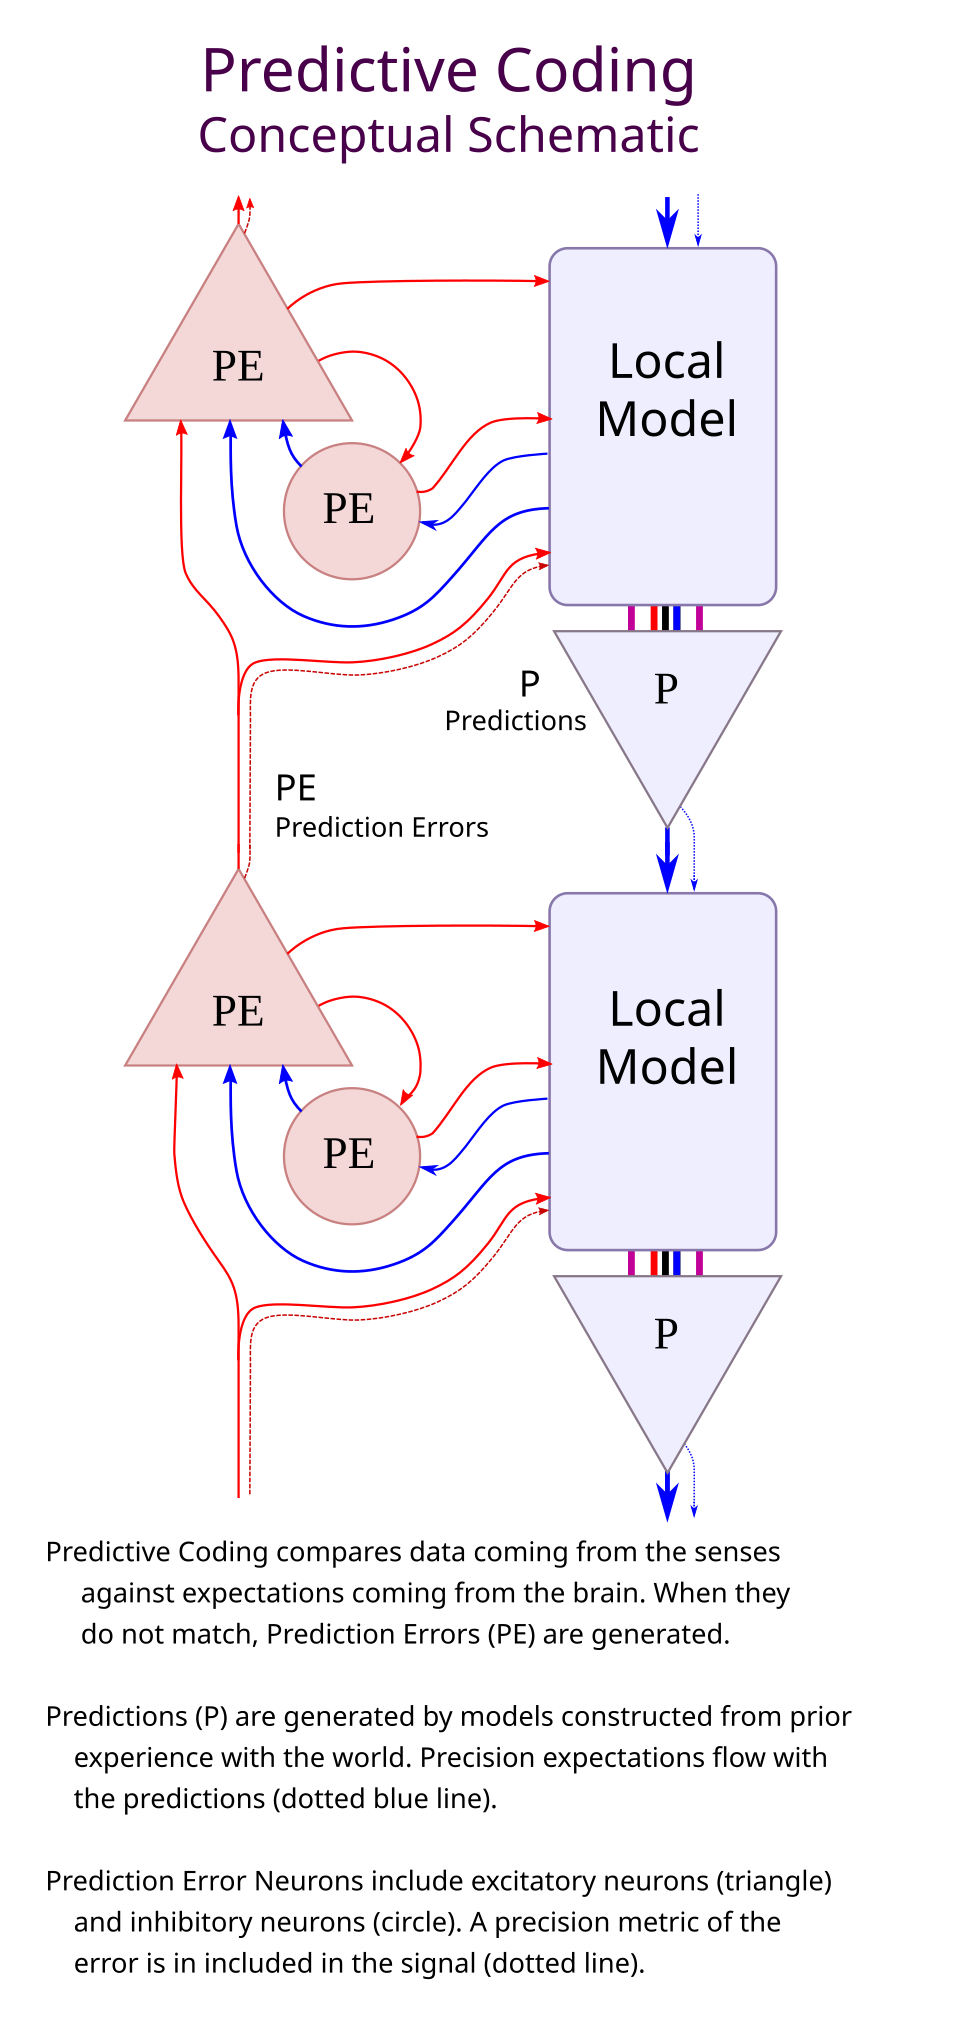
\includegraphics[width=0.9\textwidth]{predictive_coding.png}
        \end{figure}
    
    
    \section{Parts}
        
        \subsection{Local model}
        
        \subsection{Prediction model}
        
        \subsection{Prediction}
        
        \subsection{Prediction error}
    
    
    %\bibliographystyle{plainnat}
    %\bibliography{/home/donkarlo/Dropbox/repo/nd_shared_research/bibliography/bibliography.bib}
\end{document}